\chapter{Einleitung}
\pagenumbering{arabic}
\section{Aufgabenstellung gemäss Eingabe}
\label{chap:aufgabenstellung}
Im Dokument 'Bachelorthesis-Aufgabe ist' folgendes festgehalten:
\begin{quote}
Seit mehreren Jahren bestreitet die HFTM unter der Leitung von Alain Rohr mit dem Solidus Team erfolgreich die internationalen Meisterschaften des RoboCups in der 'Logistics League'.
Das Team kennt sich meisterlich mit der Ansteuerung der Hardware aus, bittet aber die BFH um Mithilfe beim Software-Engineering.
Die Aufgabe dieser Arbeit ist es, ein Software-Design für die einzelnen Komponenten des verwendeten Roboters zu entwerfen. Angelehnt an die Vorgehensweise 'Domain Driven Design' soll konkret anhand des LIDARS gezeigt werden, wie das erarbeitete Software-Design implementiert und genutzt werden soll. Folgende Merkmale soll das Design mindestens aufweisen:

\begin{itemize}
	\item Die Schnittstelle der einzelnen Domänen muss Programmiersprachen-agnostisch sein
	\item Die Domänen müssen abgekapselt und unabhängig entwickelt und getestet werden können
	\item Das Design muss klar vorsehen, dass jedes Jahr das Entwicklungsteam komplett ausgetauscht wird
\end{itemize}
Bei dieser Arbeit gilt es auch zu beachten, dass die Software-Fähigkeiten des jeweiligen Entwicklungsteams erst noch ausgebildet werden müssen, es also nötig ist, die Schnittstellen so leicht und verständlich wie möglich zu halten, um nicht eine zu steile Lernkurve als Voraussetzung zu erschaffen.
\end{quote}
Im Kapitel \ref{sec:aufgabenstellung-messbar} wird die messbare Aufgabenstellung erläutert.

\section{RoboCup}
Der RoboCup ist ein Wettbewerb, der seit 1997 jährlich ausgetragen wird \cite{wikipedia-robocup}. Ursprünglich ging es hauptsächlich darum, Roboter zu entwickeln, die gegeneinander Fussball spielen. Das langfristige Ziel dieses Wettbewerbs \cite{wikipedia-roboterfussball}: 
\begin{quote}
	im Jahr 2050 den menschlichen Weltmeister in einem gewöhnlichen Fussballspiel zu schlagen
\end{quote}
Es kommen jedoch immer neue Ligen dazu. Der aktuelle Stand an Ligen für den RoboCup 2018 ist in Screenshot aus Abbildung \ref{fig:robocup_ligen} ersichtlich.
\begin{figure}[H]
	\centering
	\includegraphics[width=\textwidth]{img/robocup/ligen.png}
	\caption{RoboCup Ligen, Screenshot von \cite{www.robocup.org}}
	\label{fig:robocup_ligen}
\end{figure} 
So gibt es beispielsweise in der Disziplin ,,RoboCupSoccer'' die Liga ,,Humanoid''. Die Roboter aus dieser Liga sind auch in den Medien hierzulande sehr bekannt. Im Bild \ref{fig:robocup_fussball} ist ein solcher Humanoid beim Fussballspielen am RoboCup zu sehen.
\begin{figure}[H]
	\centering
	\includegraphics[width=0.2\textwidth]{img/robocup/13-06-28-robocup-eindhoven-024.jpg}
	\caption{Roboter beim Fussball spielen. Foto von Ralf Roletschek / roletschek.at \cite{robocup2013}}
	\label{fig:robocup_fussball}
\end{figure}
\subsection{RoboCupLogistics}
Seit 2012 gibt es am RoboCup die Liga ,,Logistics'', die wie folgt spezifiziert ist \cite{wikipedia-robocup}:
\begin{quote}
	Ziel dieser Liga ist die Entwicklung von autonom agierender Roboter zur Steuerung des Material- und Informationsflusses in industriellen Produktionsanlagen.
\end{quote}
Es spielen zwei Teams gegeneinander mit jeweils 3 Robotern. Auf dem  Spielfeld (Abbildung \ref{fig:robocup_spielfeld}) sind pro Team zufällig sieben Maschinen  aufgestellt. Diese müssen von den Robotern erkundet werden. Dafür hat jede Maschine vorne und hinten einen eindeutigen 2D-Code aufgedruckt, dem so genannten AR Tag (Prinzip ähnlich einem QR-Code). Jede Maschine repräsentiert eine Station in einer Produktionsanlage (einer ,,smart factory''). An jeder Station können Gegenstände zugebracht und auf der gegenüberliegenden Seite entnommen werden. Kontrolliert, überwacht und bewertet wird das Spiel von der ,,Referee Box''. Von ihr werden die 'Active orders'(Bestellungen) verwaltet und publiziert, die die Roboter auf dem Spielfeld umsetzen müssen. Sie koordiniert auch die Maschinen auf dem Spielfeld, zu denen die Roboter fahren müssen, um Gegenstände zu bringen und abzuholen.
\begin{figure}[H]
	\centering
	\includegraphics[width=0.75\textwidth]{img/robocup/spielfeld_2d.png}
	\caption{Spielfeld mit möglicher Aufstellung der Maschinen: Quelle: robotics-erlangen.de \cite{robotics-erlangen.de}}
	\label{fig:robocup_spielfeld}
\end{figure}

Die verwendeten Roboter in dieser Liga basieren auf der ,,Robotino''-Plattform  von Festo, die den Wettbewerb auch mit den Maschinen und anderem sponsern. Auf dieser Roboterplattform können verschiedene Sensoren, Aktoren und Computer-Systeme angebaut werden. 
\begin{figure}[H]
	\centering
	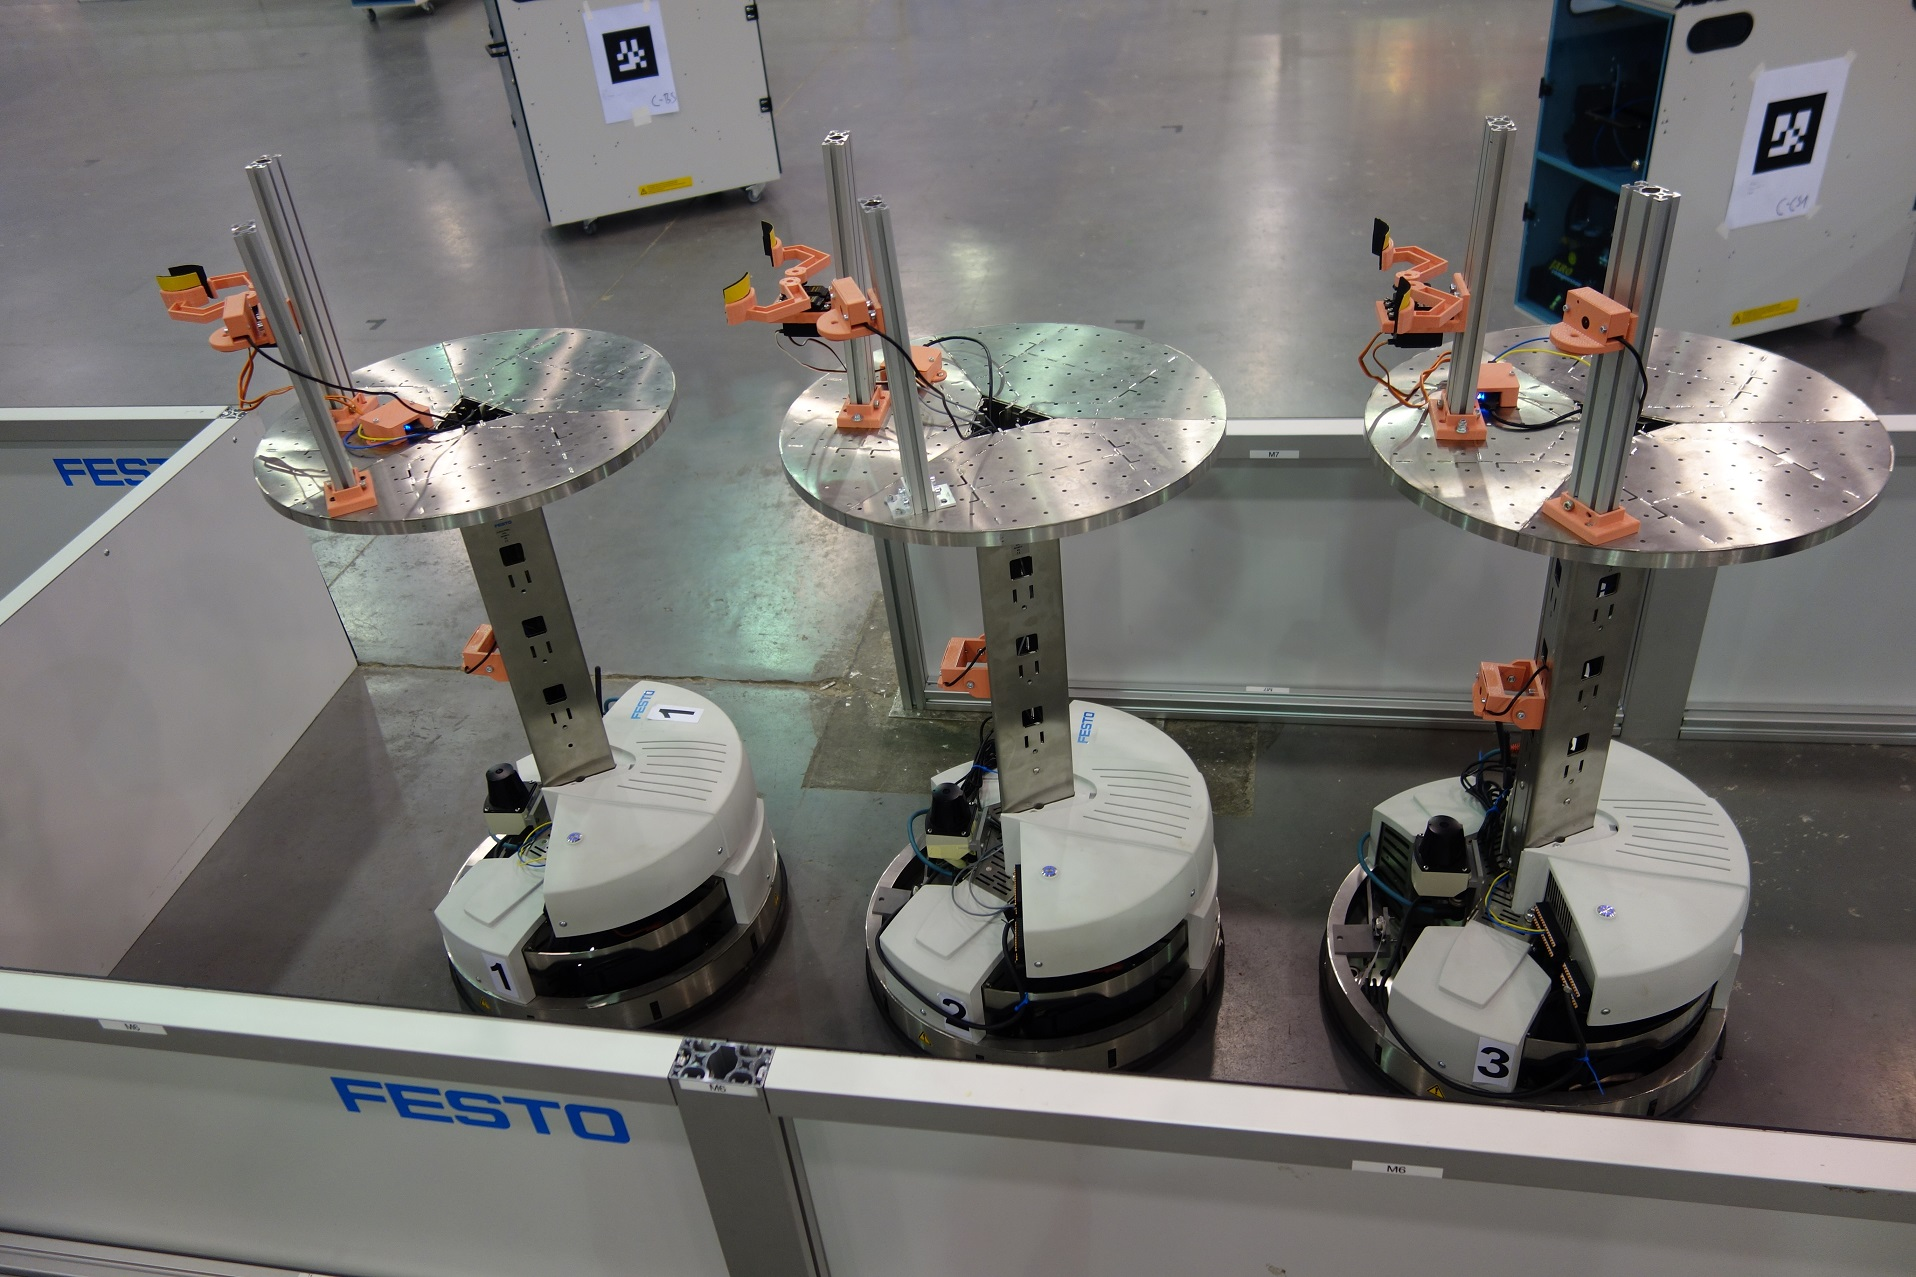
\includegraphics[width=0.5\textwidth]{img/robocup/robotino_v3.jpg}
	\caption{Robotino v3 für die Logistics League\cite{robotino}}
	\label{fig:robotino}
\end{figure}

\section{\acrfull{hftm}}
Bis anhin haben die Studenten der Höheren Fachschule für Technik Mittelland (\acrshort{hftm}) aus der Studienrichtung Systemtechnik am RoboCup unter dem Team-Namen Solidus bereits an der Spitze mitgespielt. So fragt man sich vielleicht, wieso diese Arbeit überhaupt zu Stande kommt. \\ Bis heute entwickelt man mit einem monolithischen Ansatz. Das Meiste ist eng miteinander verzahnt und die Software lässt sich schwer und mit viel Zeit weiterentwickeln. Der Roboter für den Wettbewerb wird gleichzeitig aber von Jahr zu Jahr komplexer und es müssen immer wieder Anpassungen an die neue Regeln gemacht werden und neue Dinge (Bsp. Sensoren) integriert werden. Auch müssen sich die Schüler jedes Jahr durchgehend mit allen Softwareteilen (von der Hardware-Ansteuerung bis Business-Logik) neu befassen. Die Studenten haben im Normalfall keinen Softwareentwicklungs-Hintergrund und werden parallel erst an Java ausgebildet.

\section{Lidar}
Diese Arbeit zeigt anhand eines \acrshort{lidar}-Sensors, wie ein mögliches Software-Design für den Roboter aussehen kann. Doch was ist \acrshort{lidar}?
\begin{quote}
	Lidar ist eine dem Radar verwandte Methode zur optischen Abstands- und Geschwindigkeitsmessung sowie zur Fernmessung atmosphärischer Parameter. Statt der Radiowellen wie beim Radar werden Laserstrahlen verwendet. \cite{wikipedia-lidar}
\end{quote}
Meistens versteht man unter em Begriff \acrshort{lidar} gleich einen Sensor, wie er auch in dieser Arbeit verwendet wird. Sie messen nicht nur in eine Richtung, sondern fast die ganze Umgebung um den Sensor herum. Der in dieser Arbeit verwendete TiM55x kann 270° der Umgebung ausmessen. Solche Sensoren kommen beispielsweise bei Fahrzeugen mit Autopilot (Bsp. Tesla) zum Einsatz um die Hindernisse in der Umgebung zu erkennen. Im Prinzip funktionieren solche Sensoren ähnlich wie eine Radar-Bodenstation in der Luftfahrt: Über ein drehendes Element (bei \acrshort{lidar} einen Spiegel) werden kontinuierlich Laserstrahl-Impulse ausgesendet. Wenn sich ein Objekt in der Nähe des Sensors befindet, trifft dieser Laserstrahl das Objekt und ein Teil davon wird reflektiert. Die Reflexion detektiert der Sensor und errechnet daraus die resultierende Distanz zum Objekt.
\begin{figure}[H]
	\centering
	\includegraphics[width=0.7\textwidth]{img/lidar/lidar-principle2.png}
	\caption{Prinzip 2D-Abtastung mit Lidar \cite{wikipedia-lidar}}
	\label{fig:lidar-principle}
\end{figure}


\subsection{SICK TiM55x}
\label{chap:tim55x}
Die Funktionsweise des verwendeten Sensors ist im Datenblatt vom Hersteller SICK wie folgt beschrieben \cite{tim55x-techinfo}:
\begin{quote}
Der TiM5xx sendet mit einer Laserdiode gepulste Laserstrahlen aus. Trifft ein solcher Laserpuls auf ein Objekt oder eine Person, wird er an dessen Oberfläche reflektiert. Die Reflexion wird im Empfänger des TiM5xx von einer Fotodiode registriert. Der TiM5xx nutzt die SICK-eigene HDDM-Technologie (High Definition Distance Measurement). Bei diesem Messverfahren wird ein Messwert durch die Mittelwertbildung mehrerer Einzelpulse gebildet. Aus der Laufzeit, die das Licht von der Aussendung des Strahls bis zum Empfang der Reflexion benötigt, berechnet der TiM5xx die Entfernung zum Objekt. Dieses Prinzip der ,,Pulslaufzeitmessung'' wird in ähnlicher Form von Radarsystemen benutzt.

Mit einem rotierenden Spiegel lenkt der TiM5xx die ausgesendeten Laserstrahlen ab und tastet damit die Umgebung radial ab. Die Messungen werden intern von einem Winkelkodierer in regelmässigen Winkelschritten ausgelöst. Eine komplette Rotation stellt einen Messvorgang (Scan) dar. Der TiM5xx arbeitet mit einer Scanfrequenz von 15 Hz, d. h. er durchläuft 15 Messvorgänge pro Sekunde und stellt die Messergebnisse fortlaufend in Echtzeit über die Ethernet-Schnittstelle zur Verfügung.
\end{quote}

Wir erhalten also von diesem Sensor 15 Mal Sekunde eine komplette Messung mit 270 Distanzen und der dazugehörigen Genauigkeit. Diese Messwerte sind wie im Datenblatt beschrieben wie folgt zu verstehen: Der erste Messwert erhalten wir bei -45° und der letzte bei 225° (siehe dazu Abbildung \ref{fig:lidar}). Der TiM55x-Sensor ist an der Robotino-Plattform so verbaut, dass 90° vorne entspricht. Weshalb der Hersteller negative Werte im Koordinatensystem verwendet hinterfragen wir nicht weiter. Die zu entwickelnde Software soll also genau diesen Winkel-Bereich zur Verfügung stellen - so steht er auch im Datenblatt.
\begin{figure}[H]
	\centering
	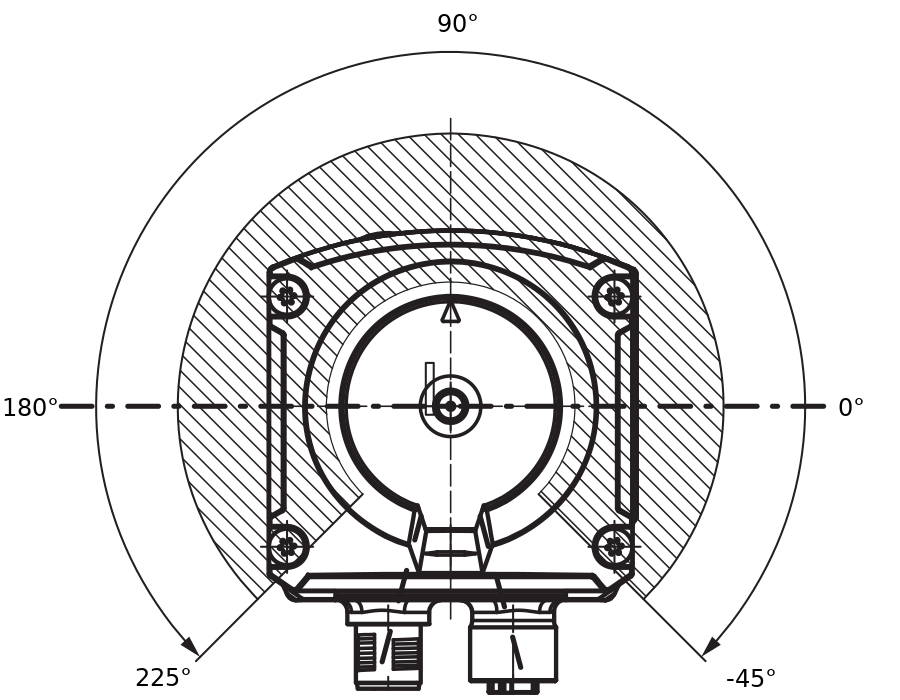
\includegraphics[width=0.5\textwidth]{img/lidar/lidar-coordinate.png}
	\caption{\acrshort{lidar}: Draufsicht / Koordinatensystem}
	\label{fig:lidar}
\end{figure}